\chapter{Background}\label{ch:background}

This chapter provides a theoretical overview of RL foundation based on \citet{sutton_reinforcement_2018}, together with specific algorithms relevant to this project. The reader is welcome to skip to the next \autoref{ch:problem_formulation} if these concepts are familiar.


\section{Markov Decision Process}

The goal of RL agent is to maximize the total reward that is accumulated during a sequential interaction with the environment. This paradigm can be expressed with a classical formulation of Markov decision process (MDP), where \autoref{fig:bg_mdp_loop} illustrates its basic interaction loop. In MDPs, actions of agent within the environment make it traverse different states and receive corresponding rewards. MDP is an extension of Markov chains, with an addition that agents are allowed to select the actions they execute. Both of these satisfy the Markov property, which assumes that each state is only dependent on the previous state, i.e.~a memoryless property where each state contains all information that is necessary to predict the next state. Therefore, MDP formulation is commonly used within the context of RL because it captures a variety of tasks that general-purpose RL algorithms can be applied to, including robotic manipulation tasks.

It should be noted that partially observable Markov decision process (POMDP) is a more accurate characterisation of most robotics tasks because the states are commonly unobservable or only partially observable, however, the difficulty of solving POMDPs limits their usage \cite{kroemer_review_2021}. Therefore, this chapter presents only on MDPs where observations and states are considered to be the same.

\begin{figure}[ht]
    \centering
    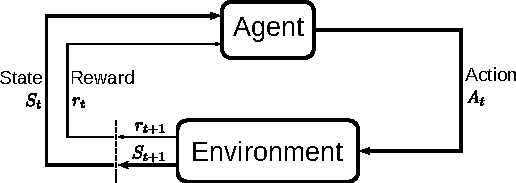
\includegraphics[width=0.75\textwidth]{background/mdp_loop.pdf}
    \caption{The interaction between agent and environment in MDP.~\protect\cite{sutton_reinforcement_2018}}
    \label{fig:bg_mdp_loop}
\end{figure}

MDPs are typically described as a tuple~\((\mathcal{S}, \mathcal{A}, p, r)\). In this work, the state space~\(\mathcal{S}\) and action space~\(\mathcal{A}\) are assumed to be continuous. The state transition probabilities are defined by function~\(p : \mathcal{S} \times \mathcal{S} \times \mathcal{A} \rightarrow [0, 1]\) that represents the probability density of the next state~\(s' \in \mathcal{S}\) based on the current state~\(s \in \mathcal{S}\) and action~\(a \in \mathcal{A}\).
\begin{equation}
    p(s' \vert s, a) = \Pr\{S_{t+1}{=}s' \vert S_{t}{=}s, A_{t}{=}a\}
\end{equation}

The behaviour of an agent is defined by a policy~\(\pi : \mathcal{S} \rightarrow \mathcal{A}\) that provides a mapping from states to actions. At each discrete time step~\(t\), the environment utilises reward function~\(r(s_{t}, a_{t})\) to emit a scalar value that expresses the immediate reward~\(r_{t} \in \mathbb{R}\) for executing action~\(a_{t}\) in state~\(s_{t}\) with policy~\(\pi\). Since both immediate and future rewards must be considered in MDP setting, the return~\(G_{t}\) that RL agent seeks to maximise is defined as a sum of discounted rewards
\begin{equation}
    G_{t} = \sum\limits_{i=t}^T \gamma^{i-t} r(s_{i}, a_{i}),
\end{equation}
where~\(\gamma \in [0, 1]\) is a discount factor that determines the priority of long-term future rewards and ensures that return is finite for continuous tasks.~\(T\) denotes a final time step, which either indicates the end of episode for episodic tasks or~\(T=\infty\) for continuous tasks. Episodic robotic grasping task with a fixed maximum number of time steps is considered in this work.

A value function can be defined to determine the expected return when following a policy~\(\pi\) for a particular state~\(s\) with value function~\(V^{\pi}(s)\). Similarly, an action-value function for taking action~\(a\) in state~\(s\) and then following policy~\(\pi\) can be defined as~\(Q^{\pi}(s, a)\).
\begin{alignat}{2}
    V^{\pi}(s)    & = \mathbb{E}_{\pi} [G_{t} \vert S_{t}{=}s]            &  & = \mathbb{E}_{\pi} \left[ \sum\limits_{i=t}^T \gamma^{i-t} r(s_{i}, a_{i}) \middle\vert\ S_{t}{=}s \right]
    \label{eq:state_value_function}                                                                                                                                                                  \\
    Q^{\pi}(s, a) & = \mathbb{E}_{\pi} [G_{t} \vert S_{t}{=}s, A_{t}{=}a] &  & = \mathbb{E}_{\pi} \left[ \sum\limits_{i=t}^T \gamma^{i-t} r(s_{i}, a_{i}) \middle\vert\ S_{t}{=}s, A_{t}{=}a \right]
    \label{eq:action_value_function}
\end{alignat}

The primary goal of the agent is to find the optimal policy~\(\pi^{*}\) that is better than or equal to all other policies. This can be achieved by estimating the corresponding optimal action-value function~\(Q^{*}(s, a)\) for all~\(s\) and~\(a\).
\begin{equation}
    Q^{*}(s, a) = \underset{\pi}{max}\ Q^{\pi}(s, a)
    \label{eq:optimal_action_value_function}
\end{equation}

This optimal action-value function satisfies Bellman equation. Intuitively, Bellman optimality equation for~\(Q^{*}(s, a)\) expresses that the value of a state is equal to the expected return for the best action~\(a'\) taken in that state.
\begin{equation}
    Q^{*}(s, a) = \mathbb{E} \left[ r_{t+1} + \gamma\ \underset{a'}{max}\ Q^{*}(s_{t+1}, a') \middle\vert\ S_{t}{=}s, A_{t}{=}a \right]
\end{equation}


\section{Model-Free Reinforcement Learning}

As previously mentioned, RL algorithms can be categorised into model-based and model-free methods, latter of which are considered in this work. Aside from this classification, there are two additional distinctions among RL algorithms that can be used to categorise them. One of these distinctions is related to the way in which data is collected during the training, separating algorithm into on-policy and off-policy. Last category is based on whether RL algorithm computes a value function or not, which differentiates them into value-based and policy-based RL. Furthermore, RL algorithms apply various exploration strategies in order to balance their trade-off between gaining more knowledge about the environment through exploration and following the current most promising direction via exploitation.

On-policy algorithms are restricted to only use data that is collected by the specific policy that is being optimised during the training. On the contrary, off-policy algorithms can be used to train an agent on any data collected by an arbitrary policy. This distinction has significant impact on RL robot learning with respect to sample efficiency. On-policy algorithms cannot reuse previous data during training because the policy keeps changing with each update. As opposed to this, off-policy RL algorithms can utilise each transition multiple times. For this, experience replay buffer \cite{mnih_human-level_2015} is commonly used to store transitions when interacting with the environment, which are then used to provide samples for updating the policy. However, on-policy algorithms generally provide better convergence guarantees during learning than off-policy methods. Despite of possible instability, off-policy algorithms are typically considered to be more suitable for complex robotic tasks due to their improved sample efficiency.


\subsection{Value-Based Methods}

Value-based methods aim to estimate the optimal state-value function~\(V^{*}(s)\) or more commonly the action-value function~\(Q^{*}(s, a)\). Once the optimal action-value function~\(Q^{*}(s, a)\) is found, the optimal policy~\(\pi^{*}\) can be followed by selecting the optimal action~\(a^{*}\) at each state~\(s\).
\begin{equation}
    a^{*}(s) = arg\ \underset{a'}{max}\ Q^{*}(s, a')
\end{equation}
Such optimisation of value function is often performed off-policy and can therefore utilise experience replay. Unfortunately, these algorithms are incompatible with continuous actions, which limits their applicability for learning robotics tasks that usually require operation in continuous domain. Exception to this are tasks that allow discretisation, e.g.~approaches described in \autoref{sec:rw_reinforcement_learning} that combine pixel-wise action space with action primitives.

Temporal difference (TD) learning is a form of value-based approach in which value function is optimised by minimising TD error~\(\delta\). For action-state value function, this error arises from a notion that the value of current state and selected action~\(Q^{\pi}(s_{t}, a_{t})\) should be equal to the reward that corresponds with this state-action pair~\(r_{t}\), plus the discounted action-value estimate of the next state and best action~\(Q^{\pi}(s_{t+1}, a^{\pi})\) that follows the policy~\(\pi\).
\begin{equation}
    \delta_{t} = r_{t} + \gamma\ \underset{a'}{max}\ Q^{\pi}(s_{t+1}, a') - Q^{\pi}(s_{t}, a_{t})
    \label{eq:td_error}
\end{equation}

Q-learning uses TD learning and in fact, the TD error for action-value function from \autoref{eq:td_error} is employed by Q-learning. With this error~\(\delta_{t}\), estimating~\(Q^{*}(s_{t}, a_{t})\) becomes an optimisation problem in the following form where~\(\alpha \in (0, 1]\) is the learning rate.
\begin{equation}
    Q^{*}(s_{t}, a_{t}) \leftarrow Q^{\pi}(s_{t}, a_{t}) + \alpha\delta_{t} = Q^{\pi}(s_{t}, a_{t}) + \alpha \left[ r_{t} + \gamma\ \underset{a'}{max}\ Q^{\pi}(s_{t+1}, a') - Q^{\pi}(s_{t}, a_{t}) \right]
\end{equation}

However, classical Q-learning is inefficient for large environments because it must consider every possible state-action pair in order to determine the optimal~\(Q^{*}(s, a)\), e.g.~by using a tabular approach. Therefore, a general function approximator can be used instead of large tables to solve these inefficiency. In deep Q-learning popularised by \citet{mnih_human-level_2015}, NNs are used to approximate the action-value function~\(Q(s, a)\). Such network can be designed to process a state as the input, and output a value for each possible action. The main difference from classical Q-learning is that optimisation of~\(Q^{*}(s, a)\) is achieved by minimising TD error~\(\delta_{t}\) with respect to parameters~\(\theta\) of the NN. Action that provides the maximum output of the NN for a given state can then be selected for subsequent execution.

The benefit of utilising NNs as a function approximator for deep Q-learning is their scalability to larger environments. However, converge to optimal solution can often be difficult to achieve due to instability. Several improvements were therefore proposed over the years to mitigate this issue. An example of improving training stability is by employing target networks \cite{mnih_human-level_2015}, where one network is used for training and a different network is used for computing TD error. This allows the target network with parameters~\(\theta'\) to provide a stable measure of error that does not significantly change on each update of unrelated state-action pairs, which would otherwise be common due to the large number of network parameters. These networks must then be regularly synchronised either via hard update, i.e.~regular copy of parameters at fixed intervals, or by applying a soft update at each step in form of Polyak averaging with hyperparameter~\(\tau \in (0, 1]\).
\begin{equation}
    \theta' = \tau \theta + (1-\tau) \theta'
\end{equation}


\subsection{Policy-Based Methods}

Instead of determining actions based on their value, policy-based methods directly optimize a stochastic policy~\(\pi\) as a probability distribution~\(\pi(a \vert s, \theta)\) that is parameterised by~\(\theta\).
\begin{equation}
    \pi(a \vert s, \theta) = \Pr\{A_{t}{=}a \vert S_{t}{=}s, \theta_{t}{=}\theta \}
\end{equation}
Following a policy is therefore based on sampling an action from this distribution given a state~\(s\). Typically,~\(\theta\) are weights and biases of NN that are optimised through gradient descent on an objective function that maximises the expected return over state-action sequences, i.e.~policy gradient methods.

Policy-based algorithms are typically on-policy and therefore less sample-efficient, yet they have better convergence properties. Furthermore, these algorithms can be directly applied to continuous action spaces without any need for discretisation, which makes them appealing for many robotics problems.


\subsection{Actor–Critic Methods}
